
\section{INTRODUCTION}

\begin{figure*}[t!]
    \centering
    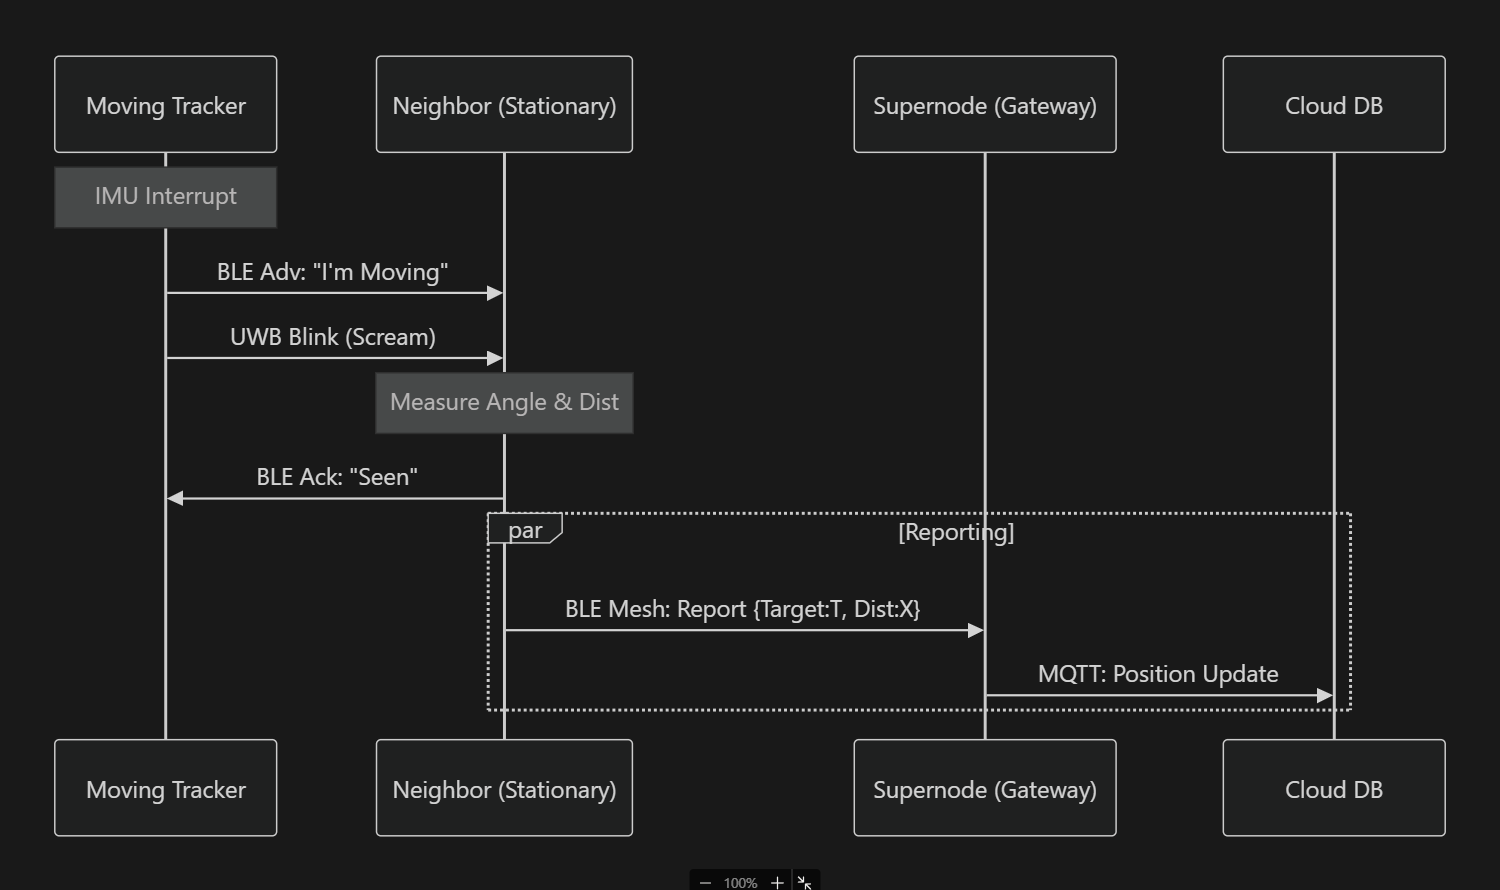
\includegraphics[width=0.9\textwidth]{images'nshi/comm.png}
    \caption{\textbf{System Overview.} The I.C.U.M. ecosystem integrates a realistic discrete-event simulator (ICUM-SIM) with a novel distributed firmware architecture. Nodes leverage event-triggered messaging (ETM) driven by inertial dynamics to maintain a rigid formation without static infrastructure, balancing localization accuracy with long-term energy efficiency.}
    \label{fig:system_overview}
\end{figure*}
%Purpose: Show how your work fits into the existing research landscape.
%Should include:
%Summaries of similar studies or technologies
%Comparisons of their strengths, limitations, or approaches
%Justification for why your method is new or necessary
\noindent Cooperative localization \cite{locatingthenodes} \cite{cooporativelocalizationinwirelessnetworks} \cite{localizationcooperative} is a localization method that uses wireless sensor nodes to leverage system architecture and network topology to estimate the positioning of these nodes. Through estimation of positions relative to each other, the nodes in the network can, with a high degree of accuracy, find the positioning of any entity within the system network. The positioning data can be either relative to each other without providing any concrete location, or, through the use of an anchor in the system architecture and topology, or coordinates computed based on the anchor coordinates and subsequent node measurements. Additionally, cooperative localization systems, being inherently distributed systems, are classified as either being centralized or decentralized \cite{wirelesssensornetworklocalizationtechniques}. The most significant differences in operational effectiveness are the tradeoffs in scalability, efficiency, and accuracy. Centralized networks are more difficult to scale properly, while decentralized networks can be less accurate and take longer to converge to a location solution.

\noindent There are mainly two techniques used to compute the distance between two nodes \cite{wirelesssensornetworklocalizationtechniques}, namely Received Signal Strength Indication (RSSI) \cite{CollaborativeLocalizationWithReceivedSignalStrengthinWirelesSensorNetworks} and Time of Flight (ToF) \cite{RadioFrequencyTimeofFlightDistanceMeasurementforLowCostWirelessSensorLocalization}. By measuring the energy exerted by a device, the strength of a radio signal can be estimated in milliwatts. Still, due to the nature of these signals, measurements become extremely small and difficult to work with. To work with these signals more easily, they are instead measured in decibel milliwatts (dBm). This non-SI logarithmic unit is measured negatively, with numbers closer to 0 indicating a stronger signal. This approach leverages any lack of synchronization between the nodes and the ubiquitous nature of technologies like Wi-Fi and Bluetooth Low Energy (BLE), which can easily measure RSS, making it great for pre-existing networks. However, RSS is extremely volatile, as a few obstacles in a non-static environment can severely impact the measured values.\\

\noindent Alternatively, UWB sensors, which are more accurate but require more power, can take advantage of ToF natively \cite{OnperformancestudyofUWBrealtimelocatingsystem}. Signals can be exchanged between two time-synchronized nodes to estimate the distance between them by comparing the time when the signal was sent by the first node and received by the second. Since radio waves travel at the speed of light, even a small difference in their clocks can lead to significant estimation errors, which means that additional computational power must be spent to ensure that all nodes are time-synchronized, a task that becomes increasingly difficult in large networks. To remedy this, UWB offers support for Two-Way Ranging (TWR), which works as stated above, but with an added message sent from the second node back to the first to calculate potential time differences \cite{Real-TimeAnchorNodeSelectionforTwo-Way-Ranging(TWR)Ultra-Wideband(UWB)IndoorPositioningSystems}.\\

\noindent Both RSS and TWR-ToF require a way to tell in which direction the measured distance is, which is done by calculating the Angle of Arrival (AoA) \cite{AnguLoc}. It’s important to note that a single UWB sensor cannot measure the AoA. It is determined by comparing the phase of the received signal across two or more antennas placed on the same UWB device, allowing the direction of the incoming signal to be estimated. Consequently, UWB nodes employing TWR-ToF were selected as the sensing technology for the cooperative localization system proposed in this paper.\\

%Cooperative localization refers to the process in which multiple agents (e.g., robots, vehicles, or sensors) estimate their positions by sharing observations and relative measurements. 
\noindent The primary advantage of cooperative localization is improved accuracy. By combining independent sensor data, agents reduce individual uncertainty and mitigate drift inherent to inertial and dead-reckoning methods \cite{CooperativeLocalizationApproachforMulti-RobotSystemsBasedonStateEstimationErrorCompensation}. Cooperative localization also enhances robustness in environments where GPS or local sensing is unreliable, since agents can provide corrective information to one another \cite{CooperativeLocalizationUsingDistanceMeasurementsforMobileNodes}. Furthermore, the approach increases fault tolerance—individual sensor failures have less impact—and supports scalability in multi-agent systems by distributing sensing responsibilities across the network \cite{Fault-TolerantMulti-ModalLocalizationofMulti-RobotsonMatrixLieGroups}. Battery performance is also a vital aspect of distributed networks if the nodes are deployed without a constant source of power. One aspect of distributed cooperative localization systems that can largely affect battery performance is the communication between nodes. Nodes that attempt to update location information despite no significant real-world change will waste a significant amount of energy \cite{EnergyEfficiencyOptimizationofCooperativeCommunicationinWirelessSensorNetworks}, while not updating location information often enough will impair the systems performance \cite{Space-TimeHierarchicalGraphBasedCooperativeLocalizationinWirelessSensorNetworks}. These two factors highlight the balance between sufficient and efficient communication needed for cooperative localization systems, which is what our research aims to achieve. Our system combines inertial movement readings to effectively detect when a location update is required. By only initiating location updating when needed, the nodes will not send superfluous location updates, and only initiate communication when needed.

\subsection*{Contributions}
\noindent This paper makes the following contributions to the field of infrastructure-free cooperative localization:
\begin{enumerate}
    \item \textbf{Event-Triggered Architecture:} We propose an IMU-gated communication protocol that reduces network overhead by over 75\% while maintaining sub-meter relative accuracy, effectively balancing energy efficiency with formation integrity.
    \item \textbf{Anchor-Free Formation Rigidity:} We demonstrate that a decentralized "spring-mass" optimization can converge to a rigid geometric formation (RMSE $< 0.1m$) solely from peer-to-peer UWB ranging, eliminating the need for expensive static infrastructure or GPS availability.
    \item \textbf{Battery-Aware Topology Control:} We introduce a hierarchical leader election algorithm that dynamically rotates cluster leadership based on energy reserves and connectivity.  Simulation results confirm this mechanism prevents the "death spiral" of critical nodes and extends the functional lifetime of the network.
    \item \textbf{Open Source Simulation Framework:} We provide ICUM-SIM, a verified component-based simulator for prototyping distributed localization algorithms with realistic physics, hardware emulation, and energy depletion models.
\end{enumerate}








